\subsection{Metodología de desarrollo}
\subsubsection{Scrum y MLOps}
MLOPS (Machine Learning Operations)\cite{MLOpsKeepCoding} y Scrum son dos enfoques diferentes pero complementarios que se pueden 
utilizar en proyectos de desarrollo de software que involucran el desarrollo de modelos de aprendizaje automático. 
Scrum es una metodología de trabajo ágil utilizado para gestionar proyectos de desarrollo de software. Se basa 
en la idea de dividir el trabajo en iteraciones cortas y enfocadas llamadas "sprints", donde se entregan incrementos 
de software funcionales al final de cada sprint. Scrum se centra en la flexibilidad, la colaboración y la capacidad 
de respuesta al cambio. Por otro lado, MLOPS se centra en la gestión del ciclo de vida del modelo, desde el 
desarrollo hasta la implementación y la puesta en producción.

\begin{figure}[ht]
    \centering
    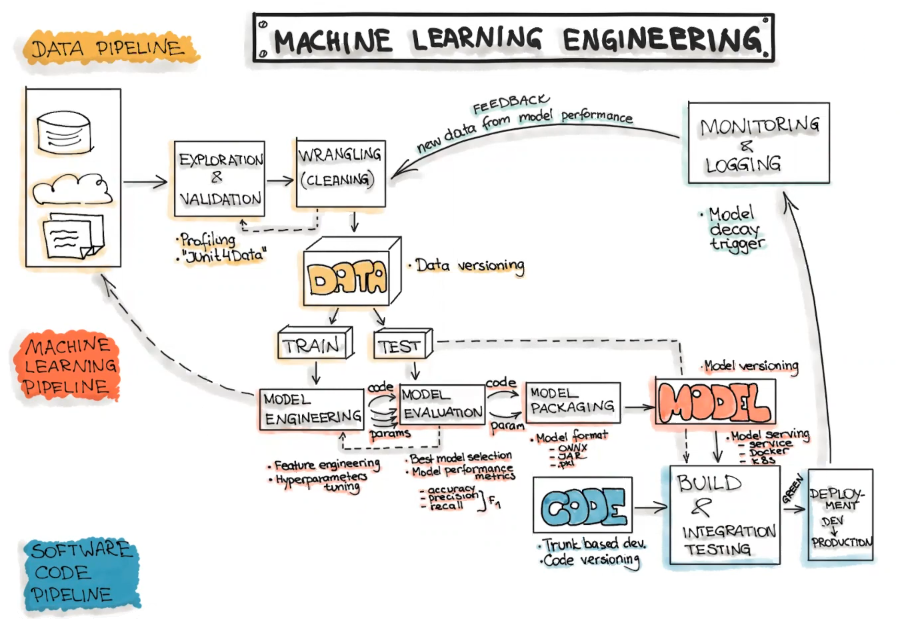
\includegraphics[scale=0.55]{architecture.png}
    \caption{Arquitectura MLOps}
    \label{fig:architecure-mlops}
\end{figure}

En este proyecto, vamos a utilizar una combinación de ambas metodologías para gestionar el desarrollo del proyecto.
Para ello vamos a recoger los principios fundamentales de Scrum y MLOps y los vamos a adaptar a nuestro proyecto.

\subsubsection{Elementos de Scrum}
A continuación, vamos a identificar aquellos elementos de Scrum esenciales para el desarrollo de nuestro proyecto.

\begin{itemize}
      \item \textbf{Planificación del sprint:} Durante la planificación del sprint en Scrum, se incluyen las
      tareas relacionadas con la recopilación y preparación de datos, la selección y entrenamiento de modelos, 
      la evaluación o implementación de la infraestructura necesaria para poner en producción los modelos.
      \item \textbf{Reuniones diarias:} Las reuniones diarias son una parte fundamental de Scrum. En estas reuniones
      se revisan las tareas realizadas, las tareas pendientes y los posibles impedimentos que puedan surgir.
      \item \textbf{Revisión del sprint:} Al final de cada sprint, se realiza una revisión del trabajo realizado
      durante el mismo.
\end{itemize}

Scrum también incluye una serie de roles:
\begin{itemize}
      \item \textbf{Product Owner:} responsable de definir las funcionalidades del producto y priorizarlas.
      \item \textbf{Scrum Master:} responsable de asegurar que el equipo de desarrollo sigue la metodología
      \item \textbf{Equipo de desarrollo:} equipo encargado de desarrollar el producto. 
\end{itemize}

En nuestro caso, el equipo de desarrollo estaría formado por el alumno, mientras que el tutor del proyecto
haría las funciones de Product Owner y Scrum Master. Más adelante, en la sección de planificación, se detallará
la lista de tareas a realizar durante el proyecto y los tiempos de desarrollo de cada una de ellas.

\subsubsection{Principios de MLOps}
A continuación, vamos a detallar los principios de MLOps que vamos a seguir en el desarrollo de nuestro proyecto.
En esta sección se incluyen los puntos más importantes de la metodología, durante todo el desarrollo intentaremos
cumplir con ellos en la medida de lo posible, ya que pueden darse situaciones en las que sea totalmente imposible
satisfacerlos al completo.

\begin{itemize}
    \item \textbf{Automatización}: la automatización es la clave para la eficiencia y el escalado.
          Aquí incluimos tareas como la generación de datos, el despliegue del modelo, la evaluación y
          la puesta en producción.
    \item \textbf{Testeo}: garantiza que tanto la funcionalidad como el desempeño del modelo están evaluados correctamente.
          Esencial en Machine Learning para identificar problemas y mejorar la confianza en los resultados.
    \item \textbf{Versionado}: es importante tener un control de versiones de los datos, el código y los modelos.
          Puede variar el método dependiendo de la herramienta que se utilice, pero existen estándares como Git para la gestión
          de código y GitHub/GitLab para el almacenamiento de los repositorios.
    \item \textbf{Reproducibilidad}: es necesario poder reproducir los resultados de forma consistente, puede ser
          complicado en Machine Learning debido a la naturaleza aleatoria de los algoritmos. Igualmente aquí se trataran
          las herramientas y medidas necesarias para lograrlo.
    \item \textbf{Monitorización}: es importante tener un control de los modelos en proceso de entrenamiento o de producción.
          Por ello, recolectar estadísticas en tiempo de procesamiento nos ayudará a generar nuevas hipótesis para las próximas 
          iteraciones.
\end{itemize}

\subsubsection{Flujo de trabajo}
Una de las características de los proyectos de Machine Learning es que son tecnologías en constante evolución, el
desarrollo no es un proceso sencillo y requiere de un enfoque coordinado por parte de los diferentes
equipos que lo conforman para asegurar su sostenibilidad a largo plazo. Es fundamental poder adaptarse a los cambios
de forma ágil, sin que esto suponga un deterioro del nivel de productividad o que ralentice el avance de nuevas
funcionalidades.\medskip

Podemos identificar tres fases principales: diseño, desarrollo del modelo y operaciones. Cada fase tiene un enfoque
específico y requiere una serie de tareas para garantizar el éxito del proyecto. La fase de diseño,
se definen los objetivos y requisitos del proyecto, se identifican los datos necesarios para el entrenamiento y
se establecen los criterios de éxito. La fase de desarrollo del modelo, se preparan los datos, se entrena el modelo
y se evalúa su rendimiento. También se realiza la validación y se toman las decisiones sobre el modelo final a utilizar.
Finalmente, en la fase de operaciones, se integra el modelo en la infraestructura existente, se monitoriza su rendimiento
y se extraen conclusiones para futuras iteraciones. Al repartir las responsabilidades en diferentes fases, aislamos los 
errores junto con la carga de trabajo y podemos avanzar sin la preocupación de que un bug o un cambio requisitos 
afecte al resto del equipo.\medskip

\begin{figure}[ht]
    \centering
    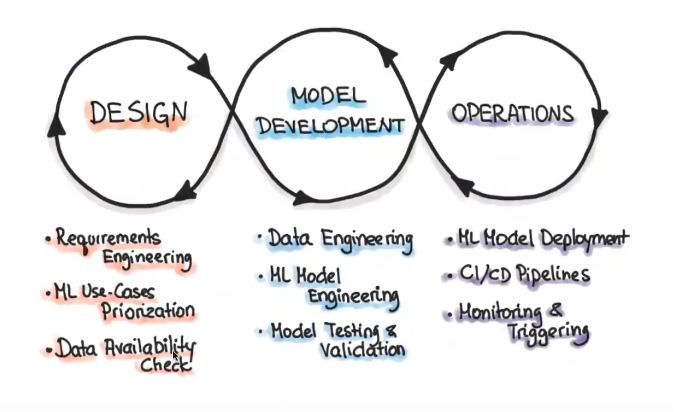
\includegraphics[scale=0.5]{proceso-mlops.png}
    \caption{Metodología MLOps}
    \label{fig:proces-mlops}
\end{figure}